The TGSN and RNN-GSN models have shown the idea so far of decoupling input representation from sequence representation. However, the sequence complexity learned still has a limit by the RNN representation capacity over the input latent space. We can generalize this decoupling idea even further by creating an alternating structure with these input representation and sequence representation layers, inspired by convolutional neural networks with alternating convolutional and dimensionality reduction layers \cite{lenet5}. The Sequence Encoder Network (SEN) is able to stack these input and sequence representational layers to learn combinations of representations for the sequence dynamics across many layers to enable a much higher capacity for complex inputs.

\section{Algorithm}

\begin{figure}[h!]
  \centering
    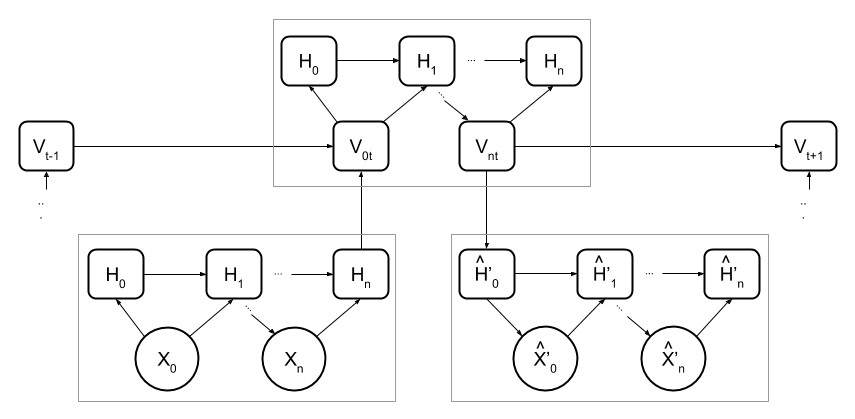
\includegraphics[width=0.8\textwidth]{sen_arch}
\caption{Sequence Encoder Network architecture. H is GSN hiddens, V is RNN hiddens.}
\end{figure}

The SEN algorithm extends the RNN-GSN by continuing to learn representations on top of the sequence representations \(V\): 
\begin{enumerate}
\item Use a GSN to learn the generative input representation \(H^0\) of the input \(X\)
\item Use an RNN to learn the sequence representation \(V^0\) over \(H^0\)
\item Use another GSN to learn \(H^1\) over the sequence representations \(V^0\)
\item Use another RNN to \(V^1\) over \(H^1\)
\item Repeat for desired representation layers \(n\) to get top-level sequence representations \(V^n\)
\end{enumerate}

Intuitively, these extra layers enable the network to represent hierarchical sequence dynamics from learning transitions between sequence representation states. This hierarchical property allows for much longer or more complex time series interactions.

The sequence representations can also be interpreted as attractor networks\cite{mathis-mozer} arranged in a hierarchical manner, learning combinations of local sequence states to form global representations. The first GSN over the learned RNN states \(V_0\) forms a localist-attractor module, where the further layered RNN and GSN hidden states reduce the dimensionality and learn increasingly global representations of the sequence state space.

Because we are essentially stacking RNN-GSN layers, the EM approach for training reconstruction and sequences separately would benefit from layerwise pretraining. For the SEN, we combine the forward passes and train both the reconstruction GSN parameters and sequence RNN parameters at the same time to avoid this issue.

While the SEN presented here uses GSN and RNN layers, it can be implemented as any encoder-decoder model that stores hidden state (VAE, convolutional autoencoder, etc.), and then any recurrent model (LSTM, GRU, etc.) to transition between hidden states used by the decoder.

 \begin{algorithm}[h!]
	\KwIn{training data \(X\) from a sequential distribution \(D\)}
	Initialize reconstruction GSN parameters \(\Theta_{gsn_n} = \) \{List(weights from one layer to the next), List(bias for layer))\} for desired layers \(n\)\;
	Initialize transition RNN parameters \(\Theta_{rnn_n} = \) \{List(weights from one layer to the next higher), List(weights from one layer to the next lower), List(bias for layer))\} for desired layers \(n\)\;
	\While{training not converged}{
		\For{each input \(X\)}{
			Run \(X\) through the SEN, creating \(H^0\) to \(H^n\) \(n*(H^i, H`^i)\) reconstruction pairs, and \(H_{t+1}^n\) expected next hiddens from the RNNs \(V^n\)\;
			Calculate the reconstruction loss for \(H\) and prediction loss for \(V\).		}
	}
	\caption{ SEN Algorithm }
\end{algorithm}



